\documentclass[xcolor=dvipsnames]{beamer} 
\usepackage[french]{babel}
\usepackage[utf8]{inputenc}
\usepackage{graphics}
\usecolortheme[named=OliveGreen]{structure} 
\useoutertheme{infolines}
\usetheme[height=7mm]{Berkeley}
\setbeamertemplate{blocks}[rounded][shadow=true] 
\setbeamertemplate{navigation symbols}{} 
\setbeamertemplate{footline}[page number]{}
\author{Lorenzo Fundaró (06-39559)\\ José Garrido (06-39590)} 
\title{Information Retrieval \\vs. \\Information Extraction} 
\institute{Universidad Simón Bolívar\\Inteligencia Artificial 2} 

\begin{document}

\begin{frame}
\titlepage
\end{frame}


\begin{frame}
\frametitle{Information Extraction - Introducción}
\begin{itemize}
 \item \textbf{Text Understanding}: \emph{El complemento de Information Retrieval}. Semántica en oraciones, inferencias implícitas, complejidad lingüística.
 \item Information Extraction se encuentra en la zona intermedia entre Information Retrieval y Text Understanding.
\end{itemize}
\begin{center}
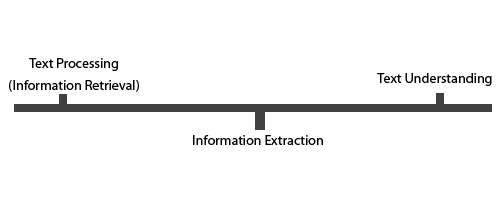
\includegraphics[scale=0.4]{IEandIR.png}
\end{center}
\end{frame}



\end{document}
